\documentclass[a4paper]{article}
\usepackage[margin=3.9cm]{geometry}
\usepackage{amsmath}
\usepackage{amssymb}
\usepackage{xcolor}
\usepackage{amsthm}
\usepackage{dsfont}
\usepackage{graphicx}
\usepackage{hyperref}
\usepackage{datetime}
\usepackage{outlines}
\usepackage{float}
\usepackage{booktabs}
\usepackage{enumitem}


\definecolor{fgcolor}{rgb}{0.345, 0.345, 0.345}
\newcommand{\hlnum}[1]{\textcolor[rgb]{0.686,0.059,0.569}{#1}}%
\newcommand{\hlstr}[1]{\textcolor[rgb]{0.192,0.494,0.8}{#1}}%
\newcommand{\hlcom}[1]{\textcolor[rgb]{0.678,0.584,0.686}{\textit{#1}}}%
\newcommand{\hlopt}[1]{\textcolor[rgb]{0,0,0}{#1}}%
\newcommand{\hlstd}[1]{\textcolor[rgb]{0.345,0.345,0.345}{#1}}%
\newcommand{\hlkwa}[1]{\textcolor[rgb]{0.161,0.373,0.58}{\textbf{#1}}}%
\newcommand{\hlkwb}[1]{\textcolor[rgb]{0.69,0.353,0.396}{#1}}%
\newcommand{\hlkwc}[1]{\textcolor[rgb]{0.333,0.667,0.333}{#1}}%
\newcommand{\hlkwd}[1]{\textcolor[rgb]{0.737,0.353,0.396}{\textbf{#1}}}%
\let\hlipl\hlkwb

\usepackage{framed}
\makeatletter
\newenvironment{kframe}{%
 \def\at@end@of@kframe{}%
 \ifinner\ifhmode%
  \def\at@end@of@kframe{\end{minipage}}%
  \begin{minipage}{\columnwidth}%
 \fi\fi%
 \def\FrameCommand##1{\hskip\@totalleftmargin \hskip-\fboxsep
 \colorbox{shadecolor}{##1}\hskip-\fboxsep
     % There is no \\@totalrightmargin, so:
     \hskip-\linewidth \hskip-\@totalleftmargin \hskip\columnwidth}%
 \MakeFramed {\advance\hsize-\width
   \@totalleftmargin\z@ \linewidth\hsize
   \@setminipage}}%
 {\par\unskip\endMakeFramed%
 \at@end@of@kframe}
\makeatother

\definecolor{shadecolor}{rgb}{.97, .97, .97}
\definecolor{messagecolor}{rgb}{0, 0, 0}
\definecolor{warningcolor}{rgb}{1, 0, 1}
\definecolor{errorcolor}{rgb}{1, 0, 0}
\newenvironment{knitrout}{}{} % an empty environment to be redefined in TeX


% code highlighting
\usepackage{minted}
\usepackage{xpatch}
\newminted[cminted]{python}{fontsize=\small}
\xpretocmd{\cminted}{\RecustomVerbatimEnvironment{Verbatim}{BVerbatim}{}}{}{}

% link coloring
%\hypersetup{
%    colorlinks,
%    linkcolor={red!80!black},
%    citecolor={green!60!black},
%    urlcolor={blue!80!black}
%}

% concatenation symbol (c.f. ++ in Haskell)
\newcommand\mdoubleplus{\mathbin{+\mkern-10mu+}}

% end of proof symbol
\newcommand{\newmarkedtheorem}[1]{%
  \newenvironment{#1}
    {\pushQED{\qed}\csname inner@#1\endcsname}
    {\popQED\csname endinner@#1\endcsname}%
  \newtheorem{inner@#1}%
}

\theoremstyle{definition}
%\newtheorem{eg}{Example}[section]
\newmarkedtheorem{eg}{Example}[section]
\newtheorem{observation}{Observation}[section]
\newtheorem{define}{Definition}[section]
\theoremstyle{plain}
\newtheorem{proposition}{Proposition}
\newtheorem{lemma}{Lemma}
\newtheorem{corollary}{Corollary}
\newtheorem{theorem}{Theorem}[section]
\newtheorem{assump}{Assumption}[section]
\newtheorem{remark}{Remark}[section]

\newdateformat{monthyeardate}{\monthname[\THEMONTH] \THEYEAR}

\author{Jeroen van Riel}
\date{\monthyeardate\today}
\title{Offline Trajectory Optimization of Autonomous Vehicles in a Single Intersection}

\begin{document}

\maketitle

\tableofcontents

\section{Problem analysis}

% general model: multi-agent optimal control problem
% derivation of the following ``offline trajectory optimization problem for a single intersection'' should happen elsewhere
% reiterate assumptions:
% (0. single intersection)
% 1. all future arrivals known
% 2. fixed routes (no dynamic rerouting)
% 3. vehicle dynamics: double integrator
% 4. central controller
This document considers the offline trajectory optimization problem for a single
intersection. Recall that \textit{offline} meant that all future arrivals to the
system are known beforehand and that we assume that routes are fixed to avoid
having to address some kind of dynamic routing problem.
In this case, we can consider the longitudinal
position $x_{i}(t)$ of each vehicle $i$ along its route, for which we use the
well-known \textit{double integrator} model
\begin{gather}
  \label{eq:vehicle_dynamics}
\begin{aligned}
  \dot{x}_{i}(t) = v_{i}(t) , \\
  \dot{v}_{i}(t) = u_{i}(t)  , \\
  0 \leq v_{\max} \leq v_{\max} , \\
  |u_{i}(t) | \leq a_{\max} ,
\end{aligned}
\end{gather}
where $v_{i}(t)$ is the vehicle's velocity and $u_{i}(t)$ its acceleration,
which is set by a single central controller. Let $D_{i}(s_{i,0})$ denote the set of all
trajectories $x_{i}(t)$ satisfying these
dynamics, given some initial state $s_{i,0} = (x_{i}(0), v_{i}(0))$.

\begin{figure}
  \centering
  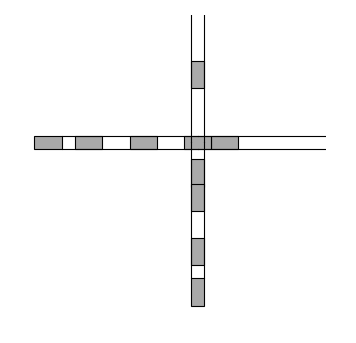
\includegraphics[width=0.4\textwidth]{figures/single_intersection_example.png}
  \caption{Illustration of a single intersection with vehicles drawn as grey
    rectangles. Vehicles approach the intersection from the east and from the
    south and cross it without turning. Note that the first two waiting vehicles
    on the south lane kept some distance before the intersection, such that they
    are able to reach full speed whenever they
    cross.}\label{fig:intersection_illustration}
\end{figure}

% model notation
Consider the single intersection illustrated in
Figure~\ref{fig:intersection_illustration}. Assume there are two incoming lanes,
identified by indices $\mathcal{R} = \{ 1, 2 \}$. The corresponding two routes
are crossing the intersection from south to north and crossing from west to
east. We identify vehicles by their route and by their relative order on this
route, by defining the vehicle index set
\begin{align}
  \mathcal{N} = \{ (r, k) : k \in \{1, \dots, n_{r}\}, r \in \mathcal{R}\} ,
\end{align}
where $n_{r}$ denotes the number of vehicles following route $r$. Smaller
values of $k$ correspond to reaching the intersection earlier. Given vehicle
index $i = (r, k) \in \mathcal{N}$, we also use the notation $r(i) = r$ and
$k(i) = k$.
%
We assume that each vehicle is represented as a rectangle of length $L$ and
width $W$ and that its position $x_{i}(t)$ is measured as the distance between
its front bumper and the start of the lane. In order to maintain a safe distance
between consecutive vehicle on the same lane, vehicle trajectories need to
satisfy
\begin{align}
  \label{eq:follow_constraints}
  x_{i}(t) - x_{j}(t) \geq L ,
\end{align}
for all $t$ and all pairs of indices $i, j \in \mathcal{N}$ such that
$r(i) = r(j), k(i) + 1 = k(j)$. Let $\mathcal{C}$ denote the set of such ordered
pairs of indices. Note that these constraints restrict vehicle from overtaking
each other, so the initial relative order is always maintained.
%
For each $i \in \mathcal{N}$, let $\mathcal{E}_{i} = (B_{i}, E_{i})$ denote the
open interval such that vehicle $i$ occupies the intersection's conflict area if
and only if $B_{i} < x_{i}(t) < E_{i}$. Using this notation, collision avoidance
at the intersection is achieved by requiring
\begin{align}
  \label{eq:conflict_constraints}
  (x_{i}(t), x_{j}(t)) \notin \mathcal{E}_{i} \times \mathcal{E}_{j} ,
\end{align}
for all $t$ and for all pairs of indices $i, j \in \mathcal{N}$ with
$r(i) \neq r(j)$, which we collect in the set $\mathcal{D}$.
%
Suppose we have some performance criterion $J(x_{i})$ that takes into account
travel time and energy efficiency of the trajectory of vehicle $i$, then the
offline trajectory optimization problem for a single intersection can be
compactly written as
\begin{subequations}
\label{eq:offline_single_intersection}
\begin{align}
  \min_{\mathbf{x}(t)} \quad & \sum_{i \in \mathcal{N}} J(x_{i}) \\
  \text{s.t.} \quad  & x_{i} \in D_{i}(s_{i,0}) , &\text{for all } i \in \mathcal{N} , \\
                & x_{i}(t) - x_{j}(t) \geq L, &\text{for all } (i,j) \in \mathcal{C} , \\
                & (x_{i}(t), x_{j}(t))  \notin \mathcal{E}_{i} \times \mathcal{E}_{j} , &\text{for all } \{i,j\} \in \mathcal{D} \label{eq:collision_constraints} ,
\end{align}
\end{subequations}
where $\mathbf{x}(t) = [\, x_{i}(t) : i \in \mathcal{N} \,]$ and constraints are
for all $t$.


\subsection{Direct transcription}

Although computationally demanding,
problem~\eqref{eq:offline_single_intersection} can be numerically solved by
direct transcription to a non-convex mixed-integer linear program by
discretization on a uniform time grid. Let $K$ denote the number of discrete
time steps and let $\Delta t$ denote the time step size.
%
Using the forward Euler integration scheme, we have
\begin{align*}
  x_{i}(t + \Delta t) = x_{i}(t) + v_{i}(t) \Delta t , \\
  v_{i}(t + \Delta t) = v_{i}(t) + u_{i}(t) \Delta t ,
\end{align*}
for each $t \in \{0, \Delta t, \dots, K \Delta t\}$. Following the approach
in~\cite{hultApproximateSolutionOptimal2015}, the collision-avoidance
constraints between lanes can be formulated using the well-known big-M technique
by the constraints
\begin{align*}
  x_{i}(t) \leq B_{i} + \delta_{i}(t) M , \\
  E_{i} - \gamma_{i}(t) M \leq x_{i}(t) , \\
  \delta_{i}(t) + \delta_{j}(t) + \gamma_{i}(t) + \gamma_{j}(t) \leq 3 ,
\end{align*}
where $\delta_{i}(t), \gamma_{i}(t) \in \{ 0, 1 \}$ for all $i \in \mathcal{N}$ and $M$ is a
sufficiently large number.
%
Finally, the follow constraints can simply be added as
\begin{align*}
  x_{i}(t) - x_{j}(t) \geq L ,
\end{align*}
for each $t \in \{0, \Delta t, \dots, K \Delta t\}$ and each pair of consecutive
vehicles $(i, j) \in \mathcal{C}$ on the same lane.
%
For example, consider the objective functional
\begin{align*}
  J(x_{i}) = \int_{t=0}^{t_{f}} \left( {(v_{d} - v_{i}(t))}^{2} + {u_{i}(t)}^{2} \right) dt ,
\end{align*}
where $v_{d}$ is some reference velocity and $t_{f}$ denotes the final time,
then the optimal trajectories are shown in
Figure~\ref{fig:direct_transcription_example}.

\begin{table}[H]
  \centering
\begin{tabular}{ c | c c c | c c }
  $i$  & (1,1) & (1,2) & (1,3) & (2,1) & (2,2) \\
  \hline
  $x_{i}(0)$ & 15 & 10 &  0 & 10 &  0 \\
  $v_{i}(0)$ & 10 & 10 & 10 & 10 & 10 \\
\end{tabular}
\caption{Example initial conditions $s_{i,0} = (x_{i}(0), v_{i}(0))$ for
  problem~\eqref{eq:offline_single_intersection}.}
\label{tab:hult_parameters}
\end{table}

\begin{figure}[t]
  \centering
  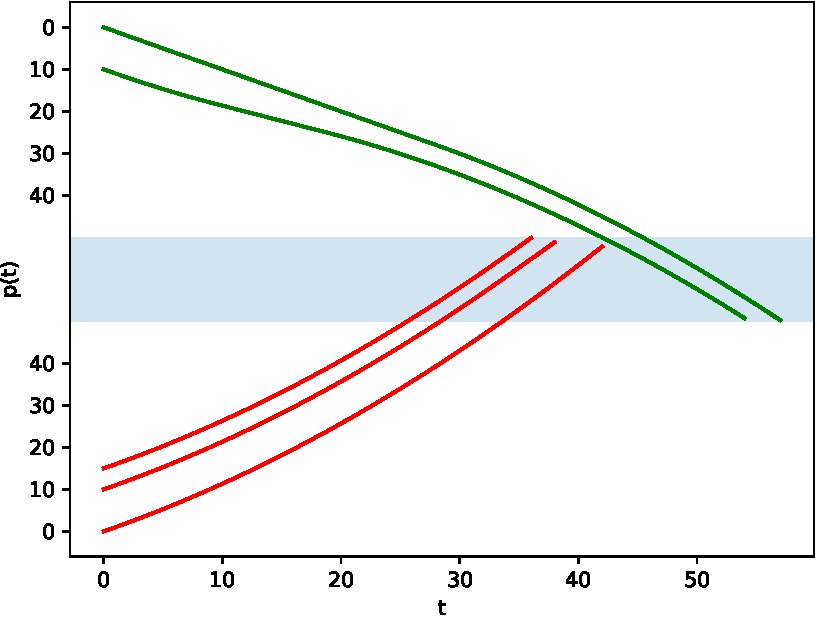
\includegraphics[width=0.7\textwidth]{figures/direct_transcription_example.pdf}
  \caption{Example of optimal trajectories obtained using the direct
    transcription method with
    $L = 5, \, \mathcal{E}_{i} \equiv \mathcal{E} = [50, 70], \, v_{d} = 20, \; T=120, \, \Delta t = 0.1$
    and initial conditions as given in Table~\ref{tab:hult_parameters}. The
    y-axis is split such that each part corresponds to one of the two lanes and
    the trajectories are inverted accordingly and drawn with separate colors.
    The intersection area $\mathcal{E}$ is drawn as a shaded region. Whenever a
    vehicle has left the intersection, we stop drawing its trajectory for
    clarity.}
  \label{fig:direct_transcription_example}
\end{figure}


\subsection{General decomposition}

For the case where only a single vehicle is approaching the intersection for
each route, so $n_{r} = 1$ for each route $r \in \mathcal{R}$, it has been shown
that problem~\eqref{eq:offline_single_intersection} can be decomposed into two coupled optimization problems, see
Theorem 1 in~\cite{hultApproximateSolutionOptimal2015}. Roughly speaking, the \textit{upper-level problem} optimizes the time
slots during which vehicles occupy the intersection, while the \textit{lower-level problem}
produces optimal safe trajectories that respect these time slots.
%
When allowing multiple vehicles per lane, we show without proof that a similar
decomposition is possible.
%
Given $x_{i}(t)$, the \textit{crossing time} of vehicle $i$, when the vehicle
first enters the intersection, and the corresponding \textit{exit time} are respectively
\begin{align}
  \inf \{ t: x_{i}(t) \in \mathcal{E}_{i} \}  \; \text{ and } \; \sup \{ t: x_{i}(t) \in \mathcal{E}_{i} \} .
\end{align}
%
The upper-level problem is to find a set of feasible occupancy timeslots, for
which the lower-level problem generates trajectories. We will use decision
variable $y(i)$ for the crossing time and write $y(i) + \sigma(i)$ for the exit
time. It turns out that trajectories can be generated separately for each route,
which yields the decomposition
%
\begin{subequations}
\begin{align}
  \min_{y, \sigma} \quad & \sum_{r \in \mathcal{R}} F(y_{r}, \sigma_{r}) \\
  \text{ s.t. } \quad & y(i) + \sigma(i) \leq y(j) \text{ or } y(j) + \sigma(j) \leq y(i), & \text{ for all } (i, j) \in \mathcal{D} , \\
  & (y_{r}, \sigma_{r}) \in \mathcal{S}_{r} , & \text{ for all } r \in \mathcal{R} ,
\end{align}
\end{subequations}
where $F(y_{r}, \sigma_{r})$ and $\mathcal{S}_{r}$ are the value function and
set of feasible parameters, respectively, of the lower-level \textit{route trajectory optimization}
problem
\begin{subequations}
\begin{align}
  F(y_{r}, \sigma_{r}) = \min_{x_{r}} \quad & \sum_{i \in \mathcal{N}(r)} J(x_{i}) \\
  \text{ s.t. } \quad & x_{i} \in D_{i}(s_{i,0}) , & \text{ for all } i \in \mathcal{N}_{r} , \\
  & x_{i}(y(i)) = B_{i} , & \text{ for all } i \in \mathcal{N}_{r} , \\
  & x_{i}(y(i) + \sigma(i)) = E_{i} , & \text{ for all } i \in \mathcal{N}_{r} , \\
  & x_{i}(t) - x_{j}(t) \geq L , & \text{ for all } (i, j) \in \mathcal{C} \cap \mathcal{N}_{r} ,
\end{align}
\end{subequations}
where we used $\mathcal{N}_{r} = \{ i \in \mathcal{N} : r(i) = r \}$ and
similarly for $x_{r}, y_{r}$ and $\sigma_{r}$ to group variables according to
route. Note that the set of feasible parameters $\mathcal{S}_{r}$ implicitly
depends on the initial states $s_{r}$ and system parameters.


\subsection{Decomposition under delay objective}

Assume that the trajectory performance criterion is exactly the crossing time,
so $J(x_{i}) = \inf \{ t: x_{i}(t) \in \mathcal{E}_{i} \}$. This assumption
makes the problem significantly easier, because we have
\begin{align}
  F(y_{r}, \sigma_{r}) \equiv F(y_{r}) = \sum_{i \in \mathcal{N}_{r}} y(i) .
\end{align}
%
Furthermore, we assume that vehicles enter the network and cross the
intersection at full speed, so $v_{i}(0) = v_{i}(y(i)) = v_{\max}$, such that we
have
\begin{align}
\sigma(i) \equiv \sigma = (L + W) / v_{\max}, \; \text{ for all } i \in \mathcal{N} .
\end{align}
%
Therefore, we ignore the part related to $\sigma$ in the set of feasible
parameters $\mathcal{S}_{r}$, which can be shown that to have a particularly
simple structure under these assumptions.
% earliest time of arrival
Observe that $r_{i} = (B_{i} - x_{i}(0)) / v_{\max}$ is the earliest time at
which vehicle $i$ can enter the intersection.
%
Let $\rho = L / v_{\max}$ be such that $y(i) + \rho$ is the time at which
the rear bumper of a crossing vehicle reaches the start line of the
intersection, then it can be shown that
$y_{r} \in \mathcal{S}_{r}$ whenever
\begin{subequations}
\begin{align}
  r_{i} \leq y(i) , & \text{ for all } i \in \mathcal{N}_{r} , \\
  y(i) + \rho \leq y(j) , & \text{ for all } (i,j) \in \mathcal{C} \cap \mathcal{N}_{r} .
\end{align}
\end{subequations}
Therefore, under the stated assumptions,
problem~\eqref{eq:offline_single_intersection} reduces to the following \textit{crossing time scheduling} problem
\begin{subequations}
  \label{eq:crossing_time_scheduling}
\begin{align}
  \min_{y} \quad & \sum_{i \in \mathcal{N}} y(i) \\
  \text{ s.t. } \quad & r_{i} \leq y(i) , & \text{ for all } i \in \mathcal{N} , \\
                    & y(i) + \rho \leq y(j) , & \text{ for all } (i,j) \in \mathcal{C} \label{eq:conjunctive} , \\
                    & y(i) + \sigma \leq y(j) \text{ or } y(j) + \sigma \leq y(i) , & \text{ for all } (i,j) \in \mathcal{D} \label{eq:disjunctive} ,
\end{align}
\end{subequations}
which can be solved using off-the-shelf mixed-integer linear program solvers,
after encoding the \textit{disjunctive constraints}~\eqref{eq:disjunctive} using
the big-M technique, which we will demonstrate in
Section~\ref{sec:branch-and-cut}. Given optimal crossing time schedule $y^{*}$, any set of trajectories
$[x_{i}(t) : i \in \mathcal{N}]$ that satisfies
\begin{subequations}
\begin{align}
  x_{i} \in D_{i}(s_{i,0}) , \quad & \text{ for all } i \in \mathcal{N} , \\
  x_{i}(y^{*}(i)) = B_{i} , \quad & \text{ for all } i \in \mathcal{N} , \\
  x_{i}(y^{*}(i) + \sigma) = E_{i} , \quad & \text{ for all } i \in \mathcal{N} , \\
  x_{i}(t) - x_{j}(t) \geq L , \quad & \text{ for all } (i,j) \in \mathcal{C} ,
\end{align}
\end{subequations}
forms a valid solution. These trajectories can be computed with an
efficient direct transcription method. First of all, note that each route may be
considered separately. Therefore, trajectories can be computed in a sequential fashion
by repeatedly solving the optimal control problem
%
\begin{align*}
\texttt{MotionSynthesize}(\tau, B, s_{0}, x') := \\
  {\arg\min}_{x: [0, \tau] \rightarrow \mathbb{R}} & \int_{0}^{\tau} |x(t)| dt \\
  \text{ s.t. } & \ddot{x}(t) = u(t) , &  \text{ for all } t \in [0, \tau] , \\
  & |u(t)| \leq a_{\max} , &  \text{ for all } t \in [0, \tau] , \\
  & 0 \leq \dot{x}(t) \leq v_{\max} , &  \text{ for all } t \in [0, \tau] , \\
  & x'(t) - x(t) \geq L , &  \text{ for all } t \in [0, \tau] , \\
  & (x(0), \dot{x}(0)) = s_{0} , \\
  & (x(\tau), \dot{x}(\tau)) = (B, v_{\max}) ,
\end{align*}
where $\tau$ is set to the required crossing time, $B$ denotes the distance to
the intersection, $s_{0}$ is the initial state of the vehicle and $x'$ denotes
the trajectory of the vehicle preceding the current vehicle.


\section{Crossing time scheduling}

Given a crossing time schedule $y$, trajectories can be efficiently computed
using a direct transcription method. Hence, we focus on solving the crossing
time scheduling problem~\ref{eq:crossing_time_scheduling}. Before we start
discussing various solution techniques, let us first introduce an alternative
way of representing instances of~\ref{eq:crossing_time_scheduling} by means of a
graph. Once we extend the current model to networks of intersection, this
encoding will be particularly helpful.

Instances and solutions of the crossing time optimization
problem~\eqref{eq:crossing_time_scheduling} can be represented by
their \textit{disjunctive graph}: let
$(\mathcal{N}, \mathcal{C}, \mathcal{O})$ be a directed graph with nodes
$\mathcal{N}$ and the following two types of arcs. The \textit{conjunctive arcs}
encode the fixed order of vehicles driving on the same lane. For each
$(i,j) \in \mathcal{C}$, an arc from $i$ to $j$ means that vehicle $i$ reaches
the intersection before $j$ due to the follow
constraints~\eqref{eq:conjunctive}. The \textit{disjunctive arcs} are used to
encode the decisions regarding the ordering of vehicles from distinct lanes,
corresponding to constraints~\eqref{eq:disjunctive}. For each pair
$\{i,j\} \in \mathcal{D}$, at most one of the arcs $(i,j)$ and $(j,i)$ can be
present in $\mathcal{O}$.

When $\mathcal{O} = \varnothing$, we say the disjunctive graph is
\textit{empty}. Each feasible schedule satisfies exactly one of the two
constraints in~\eqref{eq:disjunctive}. When $\mathcal{O}$ contains exactly one arc from every pair
of opposite disjunctive arcs, we say the disjunctive graph is \textit{complete}.
Note that such graph is acyclic and induces a unique topological ordering $\pi$
of its nodes. Conversely, every ordering $\pi$ of nodes $\mathcal{N}$ corresponds
to a unique complete disjunctive graph, which we denote by
$G(\pi) = (\mathcal{N}, \mathcal{C}, \mathcal{O}(\pi))$.

% edge weights
We define weights for every possible arc in a disjunctive graph. Every
conjunctive arc $(i, j) \in \mathcal{C}$ gets weight $w(i,j) = \rho_{i}$ and every
disjunctive arc $(i, j) \in \mathcal{O}$ gets weight $w(i,j) = \sigma_{i}$. Given
some vehicle ordering $\pi$, for every $j \in \mathcal{N}$, we recursively define
the lower bound
\begin{align}
  \text{LB}_\pi(j) = \max\{ r_{j}, \max_{i \in N^{-}_{\pi}(j)} \text{LB}_\pi(i) + w(i,j) \} ,
\end{align}
where $N^{-}_{\pi}(j)$ denotes the set of in-neighbors of node $j$ in $G(\pi)$.
Observe that this quantity is a lower bound on the crossing time, i.e., every
feasible schedule $y$ with ordering $\pi$ must satisfy $y_{i} \geq \text{LB}_\pi(i)$
for all $i \in \mathcal{N}$.
%
As the following result shows, it turns out that this lower bound is actually tight for optimal schedules,
which allows us to calculate the optimal crossing times $y^{*}$ once we know an
optimal ordering $\pi^{*}$ of vehicles, so we can concentrate on finding the latter.

\begin{proposition}\label{prop:active-schedule}
  If $y$ is an optimal schedule
  for~\eqref{eq:crossing_time_scheduling} with ordering $\pi$, then
  \begin{align}
    \label{eq:optimality}
    y_{i} = \text{\upshape LB}_{\pi}(i) \quad \text{ for all } i \in \mathcal{N} .
  \end{align}
\end{proposition}

Under the condition that $\rho_{i} = \rho$ and $\sigma_{i} = \sigma > \rho$ for all
$i \in \mathcal{N}$, it turns out that some properties of an optimal ordering can
be immediately computed from the problem specification.

\begin{proposition}\label{prop:exhaustive}
  Consider an instance of~\eqref{eq:crossing_time_scheduling} with $\rho_{i} = \rho$ and $\sigma_{i} = \sigma > \rho$ for all
  $i \in \mathcal{N}$. Suppose $y$ is an optimal schedule with
  $y_{i^{*}} + \rho \geq r_{j^{*}}$, for some $(i^{*},j^{*}) \in \mathcal{C}$, then
  $j^{*}$ follows immediately after $i^{*}$, so $y_{i^{*}} + \rho = y_{j^{*}}$.
\end{proposition}


\subsection{Branch-and-cut}
\label{sec:branch-and-cut}

Optimization problem~\ref{eq:crossing_time_scheduling} can be turned into
a Mixed-Integer Linear Program (MILP) by rewriting the disjunctive constraints using
the well-known big-M method.
%
We introduce a binary decision variable $\gamma_{ij}$ for every
disjunctive pair $\{i, j\} \in \mathcal{D}$.
%
To avoid redundant variables, we first impose some arbitrary ordering of the
disjunctive pairs by defining
\begin{align*}
  \bar{\mathcal{D}} = \{ (i,j) : \{i,j\} \in \mathcal{D}, \; l(i) < l(j) \} ,
\end{align*}
such that for every $(i,j) \in \bar{\mathcal{D}}$, setting $\gamma_{ij} = 0$
corresponds to choosing disjunctive arc $i \rightarrow j$ and
$\gamma_{ij} = 1$ corresponds to $j \rightarrow i$. This yields the following
MILP formulation
%
\begin{align*}
  \min_{y} \quad & \sum_{i \in \mathcal{N}} y_{i} & \\
  \text{s.t.} \quad & r_{i} \leq y_{i} & \text{ for all } i \in \mathcal{N} , \\
  & y_{i} + \rho_{i} \leq y_{j} & \text{ for all } (i,j) \in \mathcal{C} , \label{eq:conjunctions} \\
  & y_{i} + \sigma_{i} \leq y_{j} + \gamma_{ij}M & \text{ for all } (i,j) \in \bar{\mathcal{D}} , \\
  & y_{j} + \sigma_{j} \leq y_{i} + (1 - \gamma_{ij})M & \text{ for all } (i,j) \in \bar{\mathcal{D}} , \\
  & \gamma_{ij} \in \{0, 1\} & \text{ for all } (i,j) \in \bar{\mathcal{D}} ,
\end{align*}
where $M > 0$ is some sufficiently large number.

Consider some disjunctive arc $(i,j) \in \bar{\mathcal{D}}$. Let $i^{<}$ denote
the set of indices on lane $l(i)$ from which there is a conjunctive path to $i$.
Similarly, let $j^{>}$ denote the set of indices on lane $l(j)$ to which there is a
conjunctive path from $j$.
%
Now suppose $\gamma_{ij} = 0$, so the direction of the arc is $i \rightarrow j$,
then we must clearly also have
\begin{align*}
  p \rightarrow q \equiv \gamma_{pq} = 0 \; \text{ for all } p \in i^{<}, q \in j^{>} .
\end{align*}
Written in terms of the disjunctive variables, this gives us the cutting planes
\begin{align*}
  \sum_{p \in i^{<}, q \in j^{>}} \gamma_{pq} \leq \gamma_{ij} M .
\end{align*}
We refer to these as the \textit{disjunctive cutting planes} and any feasible solution
must satisfy these.

Next, we consider two types of cutting planes that follow from the necessary condition
for optimality in Propositon~\ref{prop:exhaustive}.
%
Suppose $y$ is an optimal schedule. If we have $y_{i} + \rho \geq r_{j}$ for
some conjunctive pair $(i,j) \in \mathcal{C}$, we must have $y_{i} + \rho = y_{j}$
by Proposition~\ref{prop:exhaustive}. In order to model this rule, we first introduce a binary
variable $\beta_{ij}$ that satisfies
\begin{align*}
  \beta_{ij} = 0 &\iff y_{i} + \rho < r_{j} , \\
  \beta_{ij} = 1 &\iff y_{i} + \rho \geq r_{j} ,
\end{align*}
which can be enforced by adding the constraints
\begin{align*}
  y_{i} + \rho &< r_{j} + \beta_{ij}M , \\
  y_{i} + \rho &\geq r_{j} - (1 - \beta_{ij}) M .
\end{align*}
Now observe that the rule is enforced by adding the following cutting plane
\begin{align*}
  y_{i} + \rho &\geq y_{j} - (1 - \beta_{ij}) M .
\end{align*}
We refer to the above cutting planes as \textit{type I}.
%
We can add more cutting planes on the disjunctive decision variables, because
whenever $\beta_{ij} = 1$, the directions of the disjunctive arcs $i \rightarrow k$ and
$j \rightarrow k$ must be the same for every other vertex $k \in \mathcal{N}$. Therefore,
consider the following constraints
\begin{align*}
  \beta_{ij} + (1 - \gamma_{ik}) + \gamma_{jk} \leq 2 , \\
  \beta_{ij} + \gamma_{ik} + (1 - \gamma_{jk}) \leq 2 ,
\end{align*}
for every $(i,j) \in \mathcal{C}$ and for every $k \in \mathcal{N}$ with $l(k) \neq l(i) = l(j)$.
These are the \textit{type II} cutting planes.

\subsection{Numerical examples}

How to define heavy-load? Formalize the situation where ``there are only two
very large platoons at the end of the schedule''.

Multimodal interarrival time distribution to model the natural occurrence of platoons.

Analyze running time of branch-and-cut and compare performance benefits of the different cutting planes.

\section{Constructive heuristics}



% constructive scheduling
Methods that rely on the branch-and-cut framework are guaranteed to find an
optimal solution, but their running time scale very badly with increasing
instance sizes. Therefore, we are interested in developing heuristics to obtain
good approximations in reasonable time. A common approach for developing such
heuristics in the scheduling literature is to try and construct a good schedule
in a step-by-step fashion. For our crossing time scheduling problem, we will
consider methods to incrementally construct a vehicle ordering, to which we will
refer as \textit{constructive heuristics}.
% introduce partial ordering and automaton model
In order to support to upcoming discussion, we first introduce some auxiliary
concepts and notation.

We define partial ordering $\pi$ to be a \textit{partial permutation} of
$\mathcal{N}$, which is a sequence of elements from some subset
$\mathcal{N}(\pi) \subset \mathcal{N}$.
%
Let $\pi$ be a partial ordering of length $n$ and let
$i \notin \mathcal{N}(\pi)$, then we use $\pi' = \pi \mdoubleplus i$ to denote
the concatenation of sequence $\pi$ with $i$, so $\pi'_{1:n} = \pi_{1:n}$ and
$\pi'_{n+1} = i$. Furthermore, let $\pi \mdoubleplus \pi'$ denote the
concatenation of two sequences $\pi$ and $\pi'$.
%
For each partial ordering $\pi$, the corresponding disjunctive graph $G(\pi)$ is
incomplete, meaning that some of the disjunctive arcs have not yet been added.
Nevertheless, observe that $\text{LB}_{\pi}(i)$ is still defined for every
$i \in \mathcal{N}$.

% lane ordering automaton
Observe that ordering vehicles is equivalent to ordering the lanes, due to the
conjunctive constraints. We will define constructive heuristics in terms of repeatedly
choosing the next lane. Hence, it may be helpful to model this process as a deterministic
finite-state automaton, where the set of lane indices acts as the input alphabet
$\Sigma = \{ 1, \dots, n \}$, where $n$ denotes the number of lanes. Let $S$
denote the state space and let $\delta: S \times \Sigma \rightarrow S$ denote
the state-transition function.
% states
Let $s$ denote an instance of~\eqref{eq:crossing_time_scheduling}. We
consider $s$ to be a fixed part of the state, so it does not change with state
transitions.
The other part of the state is the current partial ordering $\pi$.
% transitions
The transitions of the automaton are very simple. Let $(s, \pi) \in S$ denote
the current state and let $l \in \Sigma$ denote the next symbol. Let
$i \in \mathcal{N} \setminus \mathcal{N}(\pi)$ denote the next unscheduled vehicle on lane $l$,
then the system transitions to $(s, \pi \mdoubleplus i)$. If no such vehicle exists, the
transition is undefined.
%
% multi-step transition
% With a little abuse of notation, let $\delta(s, \eta) = \delta(s_{0}, \eta)$ denote the
% state that we obtain after applying sequence $\eta$ to the automaton with initial
% state $s_{0} = (s, \varnothing)$, which generalizes the single step transition function by
% recursively defining
% \begin{align*}
%   \delta(s_{0}, \eta_{1:t}) = \delta(\delta(s_{0}, \eta_{1:t-1}), \eta_{t}) .
% \end{align*}
%
Therefore, an input sequence $\eta$ of lanes is called a \textit{valid lane
  order} whenever it is of length
\begin{align*}
  N = \sum_{l \in \Sigma} n_{l}
\end{align*}
and contains precisely $n_l = |\{ i \in \mathcal{N} : l(i) = l \}|$ occurrences
of lane $l \in \Sigma$. Given problem instance $s$, let $y_{\eta}(s)$ denote the
schedule corresponding to lane order $\eta$. We say that lane order $\eta$ is
optimal whenever $y_{\eta}(s)$ is optimal. Observe that an optimal lane order
must exist for every instance $s$, since we can simply derive the lane order
from an optimal vehicle order.

Instead of mapping an instance $s$ directly to some optimal lane order, we
consider a mapping $p : S \rightarrow \Sigma$ such that setting
$s_{0} = (s, \varnothing)$ and repeatedly evaluating
\begin{align*}
  s_{t} = \delta(s_{t-1}, p(s_{t-1}))
\end{align*}
yields a final state $s_{N}(s, \pi^{*})$ with optimal schedule $\pi^{*}$.
Observe that this mapping must exist, because given some optimal lane order
$\eta^{*}$, we can set $p(s_{t}) = \eta^{*}_{t+1}$, for every $t \in \{0, \dots, N-1\}$.

We do not hope to find an explicit representation of $p$, but our aim is to find
good heuristic approximations.



\subsection{Threshold heuristics}
Consider the following simple \textit{threshold rule}.
%
Let $\pi$ denote a partial schedule of length $n$, so $i=\pi(n)$ is the last
scheduled vehicle on some lane $l=l(i)$, then define
\begin{align*}
  p_{\tau}(s, \pi) = \begin{cases}
                l \quad &\text{ if } \text{LB}_{\pi}(i) + \rho_{i} + \tau \geq r_{j} \text{ and } (i,j) \in \mathcal{C} , \\
                \texttt{next}(\pi) & \text{ otherwise, }
              \end{cases}
\end{align*}
for some threshold $\tau \geq 0$. The expression $\texttt{next}(\pi)$ represents some lane
other than $l$ with unscheduled vehicles left.

{\color{blue} Provide some examples.}
{\color{blue} Provide some intuition why this would work, using the platoon preservation theorem.}
{\color{blue} Discuss threshold tuning.}

\subsection{Neural heuristic}

{\color{blue} Provide some more introduction, explaining the intuition behind this architecture.}

We will now consider a more general class of heuristics. We model the
conditional distribution $p_{\theta}(\eta_{t+1} | s_{t})$ with model parameters
$\theta$.
%
Consider an instance $s$ and some optimal lane sequence $\eta$ with
corresponding states defined as $s_{t+1} = \delta(s_{t}, \eta_{t+1})$ for
$t \in \{0, \dots, N-1\}$. The resulting set of pairs $(s_{t}, \eta_{t+1})$ can be
used to learn $p_{\theta}$ in a supervised fashion by treating it as a classification
task.

% inference
Schedules are generated by employing \textit{greedy inference} as follows. The
model $p_{\theta}$ provides a distribution over lanes. We ignore lanes that have
no unscheduled vehicles left and take the argmax of the remaining probabilities.
We will denote the corresponding complete schedule by $\hat{y}_{\theta}(s)$.

Next, we discuss two ways of parameterizing the model. In both cases, we first
derive, for every $l \in \Sigma$, a \textit{lane embedding} $h(s_{t}, l)$ based on the current
non-final state $s_{t} = (s, \pi_{t})$ of the automaton. These are then arranged
into a \textit{state embedding} $h(s_{t})$ as follows. Let $\eta_{t}$ be the lane that was
chosen last, then we apply the following \textit{lane cycling} trick in order to keep the
most recent lane in the same position of the state embedding, by defining
\begin{align*}
  h_{l}(s_{t}) = h(s_{t}, \; l - \eta_{t} \; \mathrm{mod} \; |\Sigma|) ,
\end{align*}
for every $l \in \Sigma$.
%
This state embedding is then mapped to a probability distribution
\begin{align*}
  p_{\theta}(\eta_{t+1} | s_{t}) = f_{\theta}(h(s_{t})) ,
\end{align*}
where $f_{\theta}$ is a fully connected neural network.

{\color{blue} Include illustration of the horizons and arrows to lane embeddings.}


\subsubsection{Padded embedding}
%
Let $k_{\pi}(l)$ denote the first unscheduled vehicle in lane $l$ under the partial schedule $\pi_{t}$.
Denote the smallest lower bound of unscheduled vehicles as
\begin{align*}
  T_{\pi} = \min_{i \in \mathcal{N} \setminus \mathcal{N}(\pi)} \text{LB}_{\pi}(i) .
\end{align*}
Let the \textit{horizon} of lane $l$ be defined as
\begin{align*}
  h'(s_{t}, l) = ( \text{LB}_{\pi_{t}}(k_{\pi_{t}}(l)) - T_{\pi_{t}}, \dots, \text{LB}_{\pi_{t}}(n_{l}) - T_{\pi_{t}} ) .
\end{align*}
%
Observe that horizons can be of arbitrary dimension. Therefore, we restrict each
horizon to a fixed length $\Gamma$ and use zero padding. More precisely, given a
sequence $x = (x_{1}, \dots, x_{n})$ of length $n$, define the padding
operator
\begin{align*}
  \text{pad}(x, \Gamma) = \begin{cases}
                            (x_{1}, \dots, x_{\Gamma}) &\text{ if } \Gamma \leq n,  \\
                            (x_{1}, \dots, x_{n}) \mdoubleplus (\Gamma - n) * (0) &\text{ otherwise, }
                            \end{cases}
\end{align*}
where we use the notation $n * (0)$ to mean a sequence of $n$ zeros.
%
The lane embedding is then given by
\begin{align*}
  h(s_{t}, l) = \text{pad}(h'(s_{t}, l), \Gamma).
\end{align*}
%

\subsubsection{Recurrent embedding}

To avoid the zero padding operation, which can be problematic for states that
are almost done, we can employ a recurrent architecture that is agnostic to the
number of remaining unscheduled vehicles. Each variable-length horizon
$h'(s_{t}, l)$ is simply transformed into the fixed-length vector by an Elman
RNN by taking the output at the last step. {\color{blue} Need to further specify
  this, but the current implementation is working.}
% \begin{align*}
%   h(s_{t}, l) = \text{RNN}(h'(s_{t}, l)) .
% \end{align*}

\subsection{Comparison}

\section{Local search}

The previous section showed that constructive heuristics perform reasonably
well on average and sometimes even produce optimal solutions. To further
increase performance, without relying on the branch-and-bound framework, we
define a local search procedure.

As seen in the previous sections, vehicles of the same lane occur mostly in
groups, to which we will refer as \textit{platoons}. For example, consider example lane
order $\eta = (0, 1, 1, 0, 0, 1, 1, 1, 0, 0)$. This example has 5 platoons of
consecutive vehicles from the same lane. The second platoon consists of two
vehicles from lane 1. In general, let $P(\eta)$ denote the total number of platoons
in $\eta$.

The basic idea of our local search neighborhood is to make little changes in
these platoons by moving vehicles at the start and end of a platoon to the
previous and next platoon of the same lane.
%
More precisely, we define the following two types of modifications to a lane
order. A \textit{right-shift} modification of platoon $i$ moves the last vehicle of this
platoon to the next platoon of this lane. Similarly, a \textit{left shift} modification
of platoon $i$ moves the first vehicle of this platoon to the previous platoon
of this lane.

We construct the neighborhood of a solution by performing every possible
right-shift and left-shift with respect to every platoon in the lane order. As
an example, we have listed a full neighborhood in Table~\ref{tab:local_search}.

\newcommand*{\1}{{\color{blue}1}}%
\newcommand*{\0}{{\color{red}0}}%

\begin{table}
\begin{center}
\begin{tabular}{c|c|c}
  platoon id  & left-shift & right-shift \\
  1 &  & (\1, \1, \0, \0, \0, \1, \1, \1, \0, \0) \\
  2 & (\1, \0, \1, \0, \0, \1, \1, \1, \0, \0) & (\0, \1, \0, \0, \1, \1, \1, \1, \0, \0) \\
  3 & (\0, \0, \1, \1, \0, \1, \1, \1, \0, \0) & (\0, \1, \1, \0, \1, \1, \1, \0, \0, \0) \\
  4 & (\0, \1, \1, \1, \0, \0, \1, \1, \0, \0) & (\0, \1, \1, \0, \0, \1, \1, \0, \0, \1) \\
  5 & (\0, \1, \1, \0, \0, \0, \1, \1, \1, \0) &
\end{tabular}
\end{center}
\caption{Neighborhood of lane order $\eta = (\0, \1, \1, \0, \0, \1, \1, \1, \0, \0)$.}
\label{tab:local_search}
\end{table}

\bibliography{references}
\bibliographystyle{ieeetr}

\end{document}

% to enable the minted package
% Local Variables:
% TeX-command-extra-options: "-shell-escape"
% End:
